Para busca e persistência dos dados será utilizado a tecnologia Elasticsearch que se caracteriza por ser um mecanismo de busca open-source que realiza buscas e analisar dados em tempo real.

Baseada no Apach Lucene, Elasticsearch realizar a persistência dos dados de forma distribuída no formato de documentos os quais indexa todos os campos para que posteriormente seja possível a localização de forma rápida \cite{Gormley:2015}.

Tendo como principal objetivo facilitar a busca por texto e a rapidez no acesso aos dados e gravação, 

o Elasticsearch possui a capacidade de funcionamento escalável sendo possível a utilização em apenas um servidor (\textit{standalone}) ou de forma distribuída em centenas de servidores.
%• Capable of scaling to hundreds of servers and petabytes of structured 
Para busca é disponibilizada uma interface RESTful API que possibilita a obtenção e visualização dos dados por aplicações \textit{web client} \cite{Gormley:2015}.
%simple RESTful API, using a web client from your favorite program‐ming language, or even from the command line.  

\begin{itemize}
	\item Como esta tecnologia pode auxiliar na proposta de solução (aplicação) apresentada
\end{itemize}
\begin{figure}[!htb]
	\caption{\label{fig_grafico}JSON - Resposta da chamada a API. Comando: curl http://localhost:9200/?pretty}
	\begin{center}
		\includegraphics[width=0.6\textwidth]{imagens/pretty.eps}
	\end{center}
	\legend{Fonte: Autor}
\end{figure}
%\clearpage
